\documentclass[twoside]{book}

% Packages required by doxygen
\usepackage{calc}
\usepackage{doxygen}
\usepackage{graphicx}
\usepackage[utf8]{inputenc}
\usepackage{makeidx}
\usepackage{multicol}
\usepackage{multirow}
\usepackage{textcomp}
\usepackage[table]{xcolor}

% Font selection
\usepackage[T1]{fontenc}
\usepackage{mathptmx}
\usepackage[scaled=.90]{helvet}
\usepackage{courier}
\usepackage{amssymb}
\usepackage{sectsty}
\renewcommand{\familydefault}{\sfdefault}
\allsectionsfont{%
  \fontseries{bc}\selectfont%
  \color{darkgray}%
}
\renewcommand{\DoxyLabelFont}{%
  \fontseries{bc}\selectfont%
  \color{darkgray}%
}

% Page & text layout
\usepackage{geometry}
\geometry{%
  a4paper,%
  top=2.5cm,%
  bottom=2.5cm,%
  left=2.5cm,%
  right=2.5cm%
}
\tolerance=750
\hfuzz=15pt
\hbadness=750
\setlength{\emergencystretch}{15pt}
\setlength{\parindent}{0cm}
\setlength{\parskip}{0.2cm}
\makeatletter
\renewcommand{\paragraph}{%
  \@startsection{paragraph}{4}{0ex}{-1.0ex}{1.0ex}{%
    \normalfont\normalsize\bfseries\SS@parafont%
  }%
}
\renewcommand{\subparagraph}{%
  \@startsection{subparagraph}{5}{0ex}{-1.0ex}{1.0ex}{%
    \normalfont\normalsize\bfseries\SS@subparafont%
  }%
}
\makeatother

% Headers & footers
\usepackage{fancyhdr}
\pagestyle{fancyplain}
\fancyhead[LE]{\fancyplain{}{\bfseries\thepage}}
\fancyhead[CE]{\fancyplain{}{}}
\fancyhead[RE]{\fancyplain{}{\bfseries\leftmark}}
\fancyhead[LO]{\fancyplain{}{\bfseries\rightmark}}
\fancyhead[CO]{\fancyplain{}{}}
\fancyhead[RO]{\fancyplain{}{\bfseries\thepage}}
\fancyfoot[LE]{\fancyplain{}{}}
\fancyfoot[CE]{\fancyplain{}{}}
\fancyfoot[RE]{\fancyplain{}{\bfseries\scriptsize Generated on Thu Dec 2 2021 12\-:35\-:14 for My Project by Doxygen }}
\fancyfoot[LO]{\fancyplain{}{\bfseries\scriptsize Generated on Thu Dec 2 2021 12\-:35\-:14 for My Project by Doxygen }}
\fancyfoot[CO]{\fancyplain{}{}}
\fancyfoot[RO]{\fancyplain{}{}}
\renewcommand{\footrulewidth}{0.4pt}
\renewcommand{\chaptermark}[1]{%
  \markboth{#1}{}%
}
\renewcommand{\sectionmark}[1]{%
  \markright{\thesection\ #1}%
}

% Indices & bibliography
\usepackage{natbib}
\usepackage[titles]{tocloft}
\setcounter{tocdepth}{3}
\setcounter{secnumdepth}{5}
\makeindex

% Hyperlinks (required, but should be loaded last)
\usepackage{ifpdf}
\ifpdf
  \usepackage[pdftex,pagebackref=true]{hyperref}
\else
  \usepackage[ps2pdf,pagebackref=true]{hyperref}
\fi
\hypersetup{%
  colorlinks=true,%
  linkcolor=blue,%
  citecolor=blue,%
  unicode%
}

% Custom commands
\newcommand{\clearemptydoublepage}{%
  \newpage{\pagestyle{empty}\cleardoublepage}%
}


%===== C O N T E N T S =====

\begin{document}

% Titlepage & ToC
\hypersetup{pageanchor=false}
\pagenumbering{roman}
\begin{titlepage}
\vspace*{7cm}
\begin{center}%
{\Large My Project }\\
\vspace*{1cm}
{\large Generated by Doxygen 1.8.5}\\
\vspace*{0.5cm}
{\small Thu Dec 2 2021 12:35:14}\\
\end{center}
\end{titlepage}
\clearemptydoublepage
\tableofcontents
\clearemptydoublepage
\pagenumbering{arabic}
\hypersetup{pageanchor=true}

%--- Begin generated contents ---
\chapter{Hierarchical Index}
\section{Class Hierarchy}
This inheritance list is sorted roughly, but not completely, alphabetically\-:\begin{DoxyCompactList}
\item \contentsline{section}{I\-M\-A\-G\-E\-\_\-\-C\-L\-I\-E\-N\-T\-\_\-\-M\-S\-G}{\pageref{unionIMAGE__CLIENT__MSG}}{}
\item \contentsline{section}{I\-M\-A\-G\-E\-\_\-\-S\-E\-R\-V\-E\-R\-\_\-\-M\-S\-G}{\pageref{unionIMAGE__SERVER__MSG}}{}
\item \contentsline{section}{resolution}{\pageref{structresolution}}{}
\item \contentsline{section}{Song\-Parser}{\pageref{classSongParser}}{}
\begin{DoxyCompactList}
\item \contentsline{section}{P\-W\-M\-Song\-Parser}{\pageref{classPWMSongParser}}{}
\end{DoxyCompactList}
\item \contentsline{section}{T\-C\-P\-Client}{\pageref{classTCPClient}}{}
\begin{DoxyCompactList}
\item \contentsline{section}{Image\-Client}{\pageref{classImageClient}}{}
\end{DoxyCompactList}
\item \contentsline{section}{T\-C\-P\-Server}{\pageref{classTCPServer}}{}
\begin{DoxyCompactList}
\item \contentsline{section}{Image\-Server}{\pageref{classImageServer}}{}
\end{DoxyCompactList}
\item \contentsline{section}{timing}{\pageref{structtiming}}{}
\item Video\-Capture\begin{DoxyCompactList}
\item \contentsline{section}{Camera\-Capture}{\pageref{classCameraCapture}}{}
\end{DoxyCompactList}
\end{DoxyCompactList}

\chapter{Class Index}
\section{Class List}
Here are the classes, structs, unions and interfaces with brief descriptions\-:\begin{DoxyCompactList}
\item\contentsline{section}{\hyperlink{classCameraCapture}{Camera\-Capture} }{\pageref{classCameraCapture}}{}
\item\contentsline{section}{\hyperlink{unionIMAGE__CLIENT__MSG}{I\-M\-A\-G\-E\-\_\-\-C\-L\-I\-E\-N\-T\-\_\-\-M\-S\-G} }{\pageref{unionIMAGE__CLIENT__MSG}}{}
\item\contentsline{section}{\hyperlink{unionIMAGE__SERVER__MSG}{I\-M\-A\-G\-E\-\_\-\-S\-E\-R\-V\-E\-R\-\_\-\-M\-S\-G} }{\pageref{unionIMAGE__SERVER__MSG}}{}
\item\contentsline{section}{\hyperlink{classImageClient}{Image\-Client} }{\pageref{classImageClient}}{}
\item\contentsline{section}{\hyperlink{classImageServer}{Image\-Server} }{\pageref{classImageServer}}{}
\item\contentsline{section}{\hyperlink{classPWMSongParser}{P\-W\-M\-Song\-Parser} }{\pageref{classPWMSongParser}}{}
\item\contentsline{section}{\hyperlink{structresolution}{resolution} }{\pageref{structresolution}}{}
\item\contentsline{section}{\hyperlink{classSongParser}{Song\-Parser} }{\pageref{classSongParser}}{}
\item\contentsline{section}{\hyperlink{classTCPClient}{T\-C\-P\-Client} }{\pageref{classTCPClient}}{}
\item\contentsline{section}{\hyperlink{classTCPServer}{T\-C\-P\-Server} }{\pageref{classTCPServer}}{}
\item\contentsline{section}{\hyperlink{structtiming}{timing} }{\pageref{structtiming}}{}
\end{DoxyCompactList}

\chapter{Class Documentation}
\hypertarget{classCameraCapture}{\section{Camera\-Capture Class Reference}
\label{classCameraCapture}\index{Camera\-Capture@{Camera\-Capture}}
}
Inheritance diagram for Camera\-Capture\-:\begin{figure}[H]
\begin{center}
\leavevmode
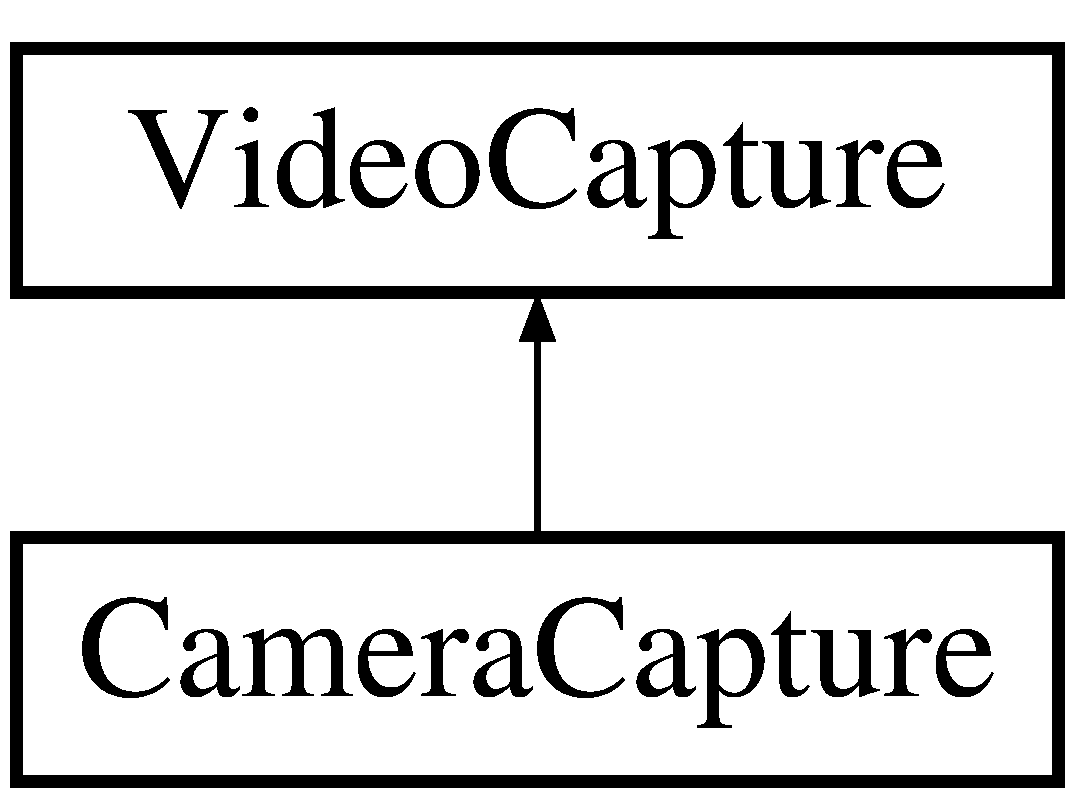
\includegraphics[height=2.000000cm]{classCameraCapture}
\end{center}
\end{figure}
\subsection*{Public Member Functions}
\begin{DoxyCompactItemize}
\item 
\hypertarget{classCameraCapture_a91c991b748f6206c84f50f5f0840532e}{void {\bfseries set\-Resolution} (uint32\-\_\-t I\-D\-\_\-\-R\-E\-S\-O\-L\-U\-T\-I\-O\-N)}\label{classCameraCapture_a91c991b748f6206c84f50f5f0840532e}

\end{DoxyCompactItemize}


The documentation for this class was generated from the following files\-:\begin{DoxyCompactItemize}
\item 
include/Camera\-Capture.\-h\item 
src/Camera\-Capture.\-cpp\end{DoxyCompactItemize}

\hypertarget{unionIMAGE__CLIENT__MSG}{\section{I\-M\-A\-G\-E\-\_\-\-C\-L\-I\-E\-N\-T\-\_\-\-M\-S\-G Union Reference}
\label{unionIMAGE__CLIENT__MSG}\index{I\-M\-A\-G\-E\-\_\-\-C\-L\-I\-E\-N\-T\-\_\-\-M\-S\-G@{I\-M\-A\-G\-E\-\_\-\-C\-L\-I\-E\-N\-T\-\_\-\-M\-S\-G}}
}
\subsection*{Public Attributes}
\begin{DoxyCompactItemize}
\item 
\hypertarget{unionIMAGE__CLIENT__MSG_a82469bd2405ba9f641fbb540b32845be}{\begin{tabbing}
xx\=xx\=xx\=xx\=xx\=xx\=xx\=xx\=xx\=\kill
struct \{\\
\>uint32\_t {\bfseries OK}: 1\\
\>uint32\_t {\bfseries QUIT}: 1\\
\>uint32\_t {\bfseries RES}: 2\\
\} {\bfseries f}}\label{unionIMAGE__CLIENT__MSG_a82469bd2405ba9f641fbb540b32845be}
\\

\end{tabbing}\item 
\hypertarget{unionIMAGE__CLIENT__MSG_a2500a5a095a7ce7b9b811c1074dc1368}{uint32\-\_\-t {\bfseries raw\-Data}}\label{unionIMAGE__CLIENT__MSG_a2500a5a095a7ce7b9b811c1074dc1368}

\end{DoxyCompactItemize}


The documentation for this union was generated from the following file\-:\begin{DoxyCompactItemize}
\item 
include/common.\-h\end{DoxyCompactItemize}

\hypertarget{unionIMAGE__SERVER__MSG}{\section{I\-M\-A\-G\-E\-\_\-\-S\-E\-R\-V\-E\-R\-\_\-\-M\-S\-G Union Reference}
\label{unionIMAGE__SERVER__MSG}\index{I\-M\-A\-G\-E\-\_\-\-S\-E\-R\-V\-E\-R\-\_\-\-M\-S\-G@{I\-M\-A\-G\-E\-\_\-\-S\-E\-R\-V\-E\-R\-\_\-\-M\-S\-G}}
}
\subsection*{Public Attributes}
\begin{DoxyCompactItemize}
\item 
\hypertarget{unionIMAGE__SERVER__MSG_a0470a6c5960e4401e73543a8df6e3f29}{\begin{tabbing}
xx\=xx\=xx\=xx\=xx\=xx\=xx\=xx\=xx\=\kill
struct \{\\
\>uint32\_t {\bfseries READY}: 1\\
\>uint32\_t {\bfseries IDOWN}: 1\\
\>uint32\_t {\bfseries PUSHB}: 1\\
\} {\bfseries f}}\label{unionIMAGE__SERVER__MSG_a0470a6c5960e4401e73543a8df6e3f29}
\\

\end{tabbing}\item 
\hypertarget{unionIMAGE__SERVER__MSG_a1eae8e211658e29ec7e3ae519df018e1}{uint32\-\_\-t {\bfseries raw\-Data}}\label{unionIMAGE__SERVER__MSG_a1eae8e211658e29ec7e3ae519df018e1}

\end{DoxyCompactItemize}


The documentation for this union was generated from the following file\-:\begin{DoxyCompactItemize}
\item 
include/common.\-h\end{DoxyCompactItemize}

\hypertarget{classImageClient}{\section{Image\-Client Class Reference}
\label{classImageClient}\index{Image\-Client@{Image\-Client}}
}


{\ttfamily \#include $<$Image\-Client.\-h$>$}

Inheritance diagram for Image\-Client\-:\begin{figure}[H]
\begin{center}
\leavevmode
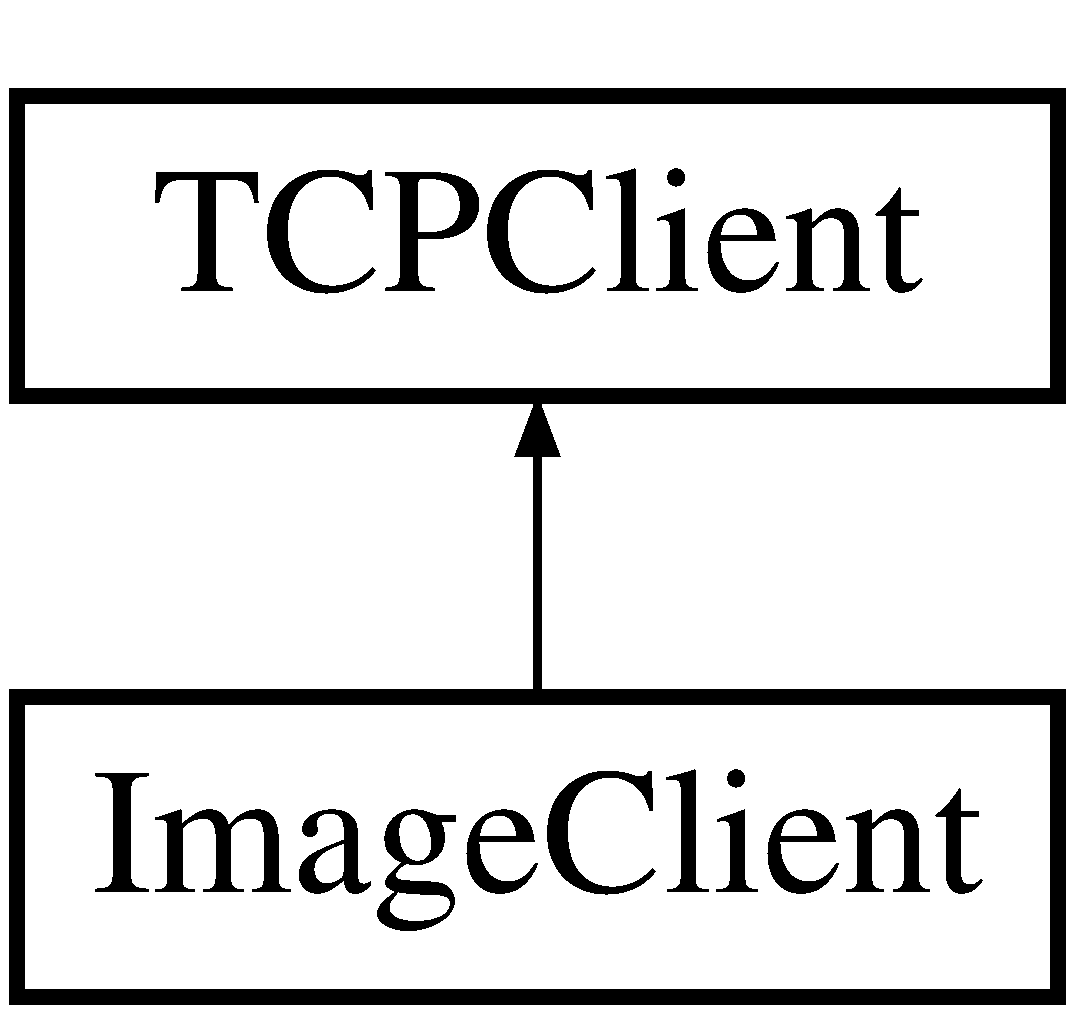
\includegraphics[height=2.000000cm]{classImageClient}
\end{center}
\end{figure}
\subsection*{Public Member Functions}
\begin{DoxyCompactItemize}
\item 
\hypertarget{classImageClient_aad4a7ff2206d2634926008ff8f710ee1}{{\bfseries Image\-Client} (int serv\-\_\-port, std\-::string serv\-\_\-addr)}\label{classImageClient_aad4a7ff2206d2634926008ff8f710ee1}

\item 
\hypertarget{classImageClient_a9d9f83083fda76d517215e810697501d}{\hyperlink{unionIMAGE__CLIENT__MSG}{I\-M\-A\-G\-E\-\_\-\-C\-L\-I\-E\-N\-T\-\_\-\-M\-S\-G} {\bfseries compute\-Message} (int key)}\label{classImageClient_a9d9f83083fda76d517215e810697501d}

\end{DoxyCompactItemize}


\subsection{Detailed Description}
\textbackslash{} class \hyperlink{classImageClient}{Image\-Client} \hyperlink{classImageClient}{Image\-Client} est une classe héritant de \hyperlink{classTCPClient}{T\-C\-P\-Client} (permettant la gestion de la connexion T\-C\-P/\-I\-P du côté client) et fournissant en plus une méthode pour envoyer les messages client. 

The documentation for this class was generated from the following files\-:\begin{DoxyCompactItemize}
\item 
include/Image\-Client.\-h\item 
src/Image\-Client.\-cpp\end{DoxyCompactItemize}

\hypertarget{classImageServer}{\section{Image\-Server Class Reference}
\label{classImageServer}\index{Image\-Server@{Image\-Server}}
}
Inheritance diagram for Image\-Server\-:\begin{figure}[H]
\begin{center}
\leavevmode
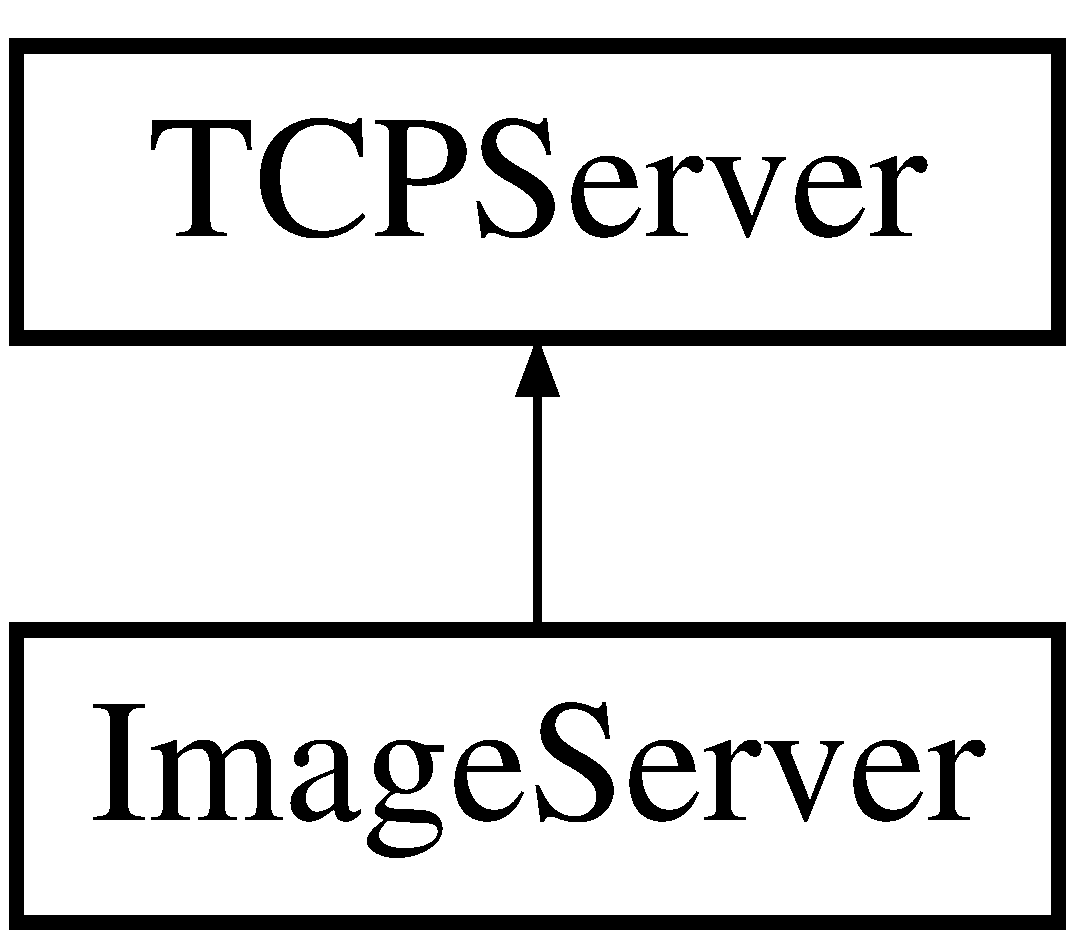
\includegraphics[height=2.000000cm]{classImageServer}
\end{center}
\end{figure}
\subsection*{Public Member Functions}
\begin{DoxyCompactItemize}
\item 
\hypertarget{classImageServer_a4b824c5337974577e55c68c3443939c6}{{\bfseries Image\-Server} (int port)}\label{classImageServer_a4b824c5337974577e55c68c3443939c6}

\item 
\hypertarget{classImageServer_ade5594050e37e16139e6707f3e8373d0}{\hyperlink{unionIMAGE__SERVER__MSG}{I\-M\-A\-G\-E\-\_\-\-S\-E\-R\-V\-E\-R\-\_\-\-M\-S\-G} {\bfseries compute\-Message} ()}\label{classImageServer_ade5594050e37e16139e6707f3e8373d0}

\end{DoxyCompactItemize}
\subsection*{Static Public Member Functions}
\begin{DoxyCompactItemize}
\item 
\hypertarget{classImageServer_a9d05ecf0fcf25972973010d5aae92cd7}{static int {\bfseries read\-File} (std\-::string file\-Path)}\label{classImageServer_a9d05ecf0fcf25972973010d5aae92cd7}

\end{DoxyCompactItemize}


The documentation for this class was generated from the following files\-:\begin{DoxyCompactItemize}
\item 
include/Image\-Server.\-h\item 
src/Image\-Server.\-cpp\end{DoxyCompactItemize}

\hypertarget{classPWMSongParser}{\section{P\-W\-M\-Song\-Parser Class Reference}
\label{classPWMSongParser}\index{P\-W\-M\-Song\-Parser@{P\-W\-M\-Song\-Parser}}
}
Inheritance diagram for P\-W\-M\-Song\-Parser\-:\begin{figure}[H]
\begin{center}
\leavevmode
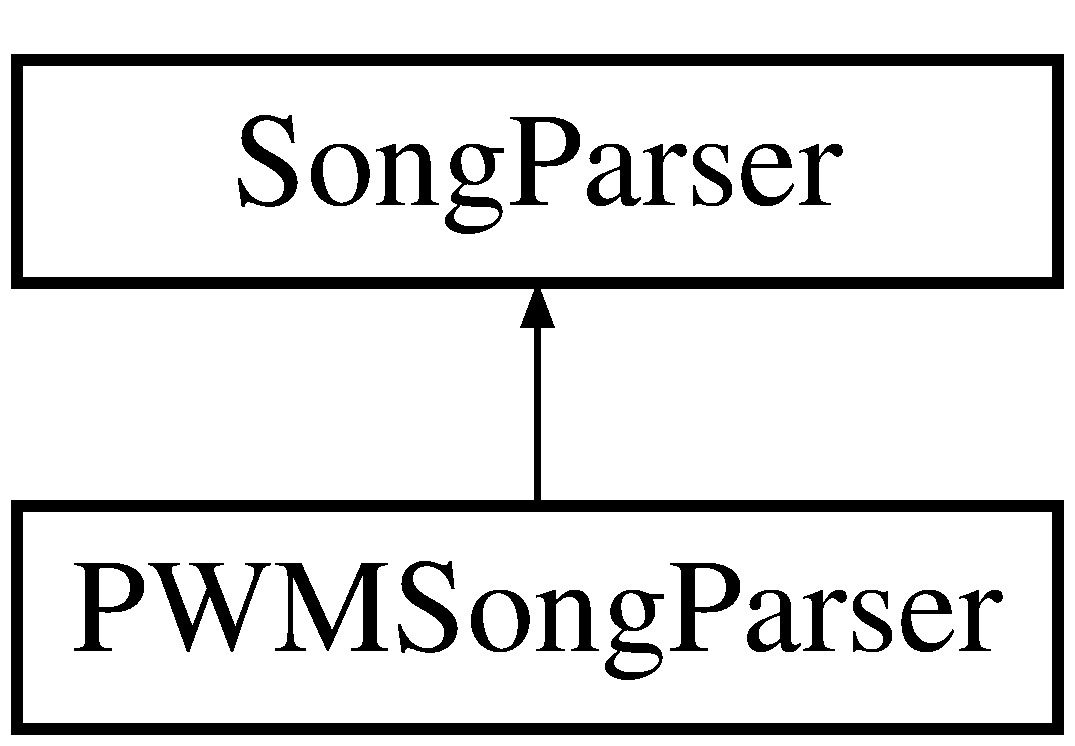
\includegraphics[height=2.000000cm]{classPWMSongParser}
\end{center}
\end{figure}
\subsection*{Public Attributes}
\begin{DoxyCompactItemize}
\item 
\hypertarget{classPWMSongParser_ab6ef175e8f80211c9648494677128e9e}{std\-::string {\bfseries frequency\-Path}}\label{classPWMSongParser_ab6ef175e8f80211c9648494677128e9e}

\item 
\hypertarget{classPWMSongParser_af5feb204b64739f4c24b5cb5637fcc4f}{std\-::string {\bfseries enable\-Path}}\label{classPWMSongParser_af5feb204b64739f4c24b5cb5637fcc4f}

\end{DoxyCompactItemize}
\subsection*{Additional Inherited Members}


The documentation for this class was generated from the following files\-:\begin{DoxyCompactItemize}
\item 
include/P\-W\-M\-Song\-Parser.\-h\item 
src/P\-W\-M\-Song\-Parser.\-cpp\end{DoxyCompactItemize}

\hypertarget{structresolution}{\section{resolution Struct Reference}
\label{structresolution}\index{resolution@{resolution}}
}
\subsection*{Public Attributes}
\begin{DoxyCompactItemize}
\item 
\hypertarget{structresolution_ad0c45ccf2d99f482f3c31138822fdcaf}{int {\bfseries x}}\label{structresolution_ad0c45ccf2d99f482f3c31138822fdcaf}

\item 
\hypertarget{structresolution_ab1fc0e14f43778ee8e25710611cdee8a}{int {\bfseries y}}\label{structresolution_ab1fc0e14f43778ee8e25710611cdee8a}

\end{DoxyCompactItemize}


The documentation for this struct was generated from the following file\-:\begin{DoxyCompactItemize}
\item 
include/Camera\-Capture.\-h\end{DoxyCompactItemize}

\hypertarget{classSongParser}{\section{Song\-Parser Class Reference}
\label{classSongParser}\index{Song\-Parser@{Song\-Parser}}
}
Inheritance diagram for Song\-Parser\-:\begin{figure}[H]
\begin{center}
\leavevmode
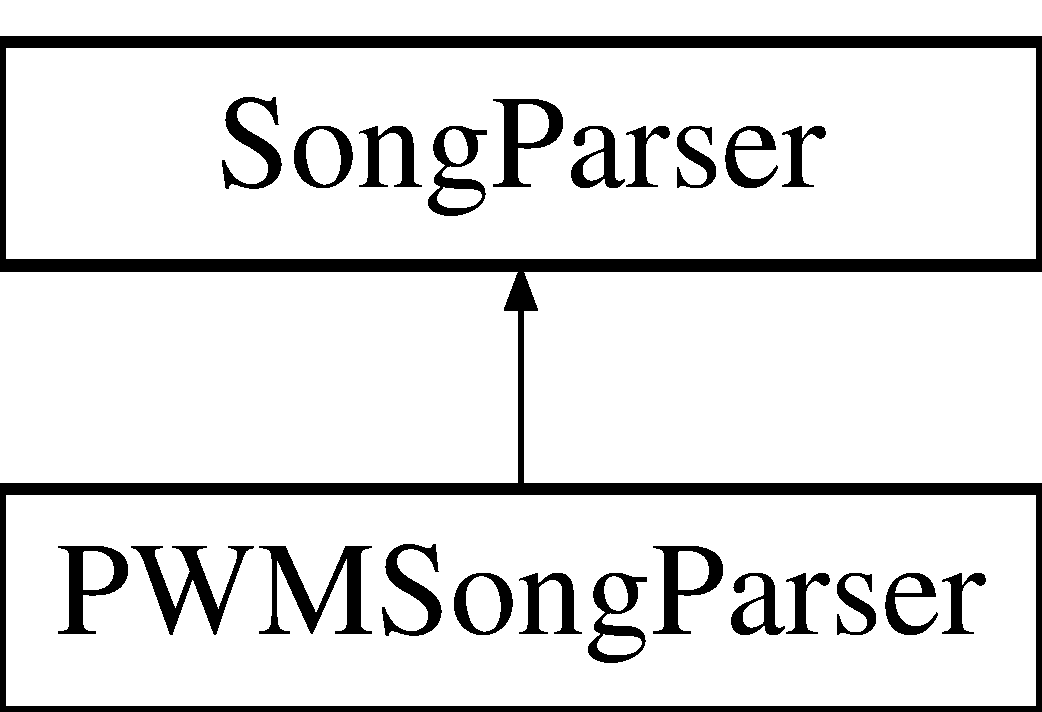
\includegraphics[height=2.000000cm]{classSongParser}
\end{center}
\end{figure}
\subsection*{Public Member Functions}
\begin{DoxyCompactItemize}
\item 
\hypertarget{classSongParser_a744cd4ea2db31242c765c3cf1968eba2}{void {\bfseries read\-String} (std\-::string song)}\label{classSongParser_a744cd4ea2db31242c765c3cf1968eba2}

\item 
\hypertarget{classSongParser_a9e10d549966c5140b9d15ffde542a9ca}{virtual void {\bfseries play} () const }\label{classSongParser_a9e10d549966c5140b9d15ffde542a9ca}

\end{DoxyCompactItemize}
\subsection*{Protected Member Functions}
\begin{DoxyCompactItemize}
\item 
\hypertarget{classSongParser_a9de796d5cbc1cbe55181a80250a6bea9}{const std\-::vector$<$ command $>$ \& {\bfseries get\-Commands} () const }\label{classSongParser_a9de796d5cbc1cbe55181a80250a6bea9}

\item 
\hypertarget{classSongParser_a5cf22619c27fb0304e635d11bbeb0d6d}{virtual void {\bfseries tone} (uint32\-\_\-t frequency, uint32\-\_\-t length) const }\label{classSongParser_a5cf22619c27fb0304e635d11bbeb0d6d}

\end{DoxyCompactItemize}


The documentation for this class was generated from the following files\-:\begin{DoxyCompactItemize}
\item 
include/Song\-Parser.\-h\item 
src/Song\-Parser.\-cpp\end{DoxyCompactItemize}

\hypertarget{classTCPClient}{\section{T\-C\-P\-Client Class Reference}
\label{classTCPClient}\index{T\-C\-P\-Client@{T\-C\-P\-Client}}
}


{\ttfamily \#include $<$T\-C\-P\-Client.\-h$>$}

Inheritance diagram for T\-C\-P\-Client\-:\begin{figure}[H]
\begin{center}
\leavevmode
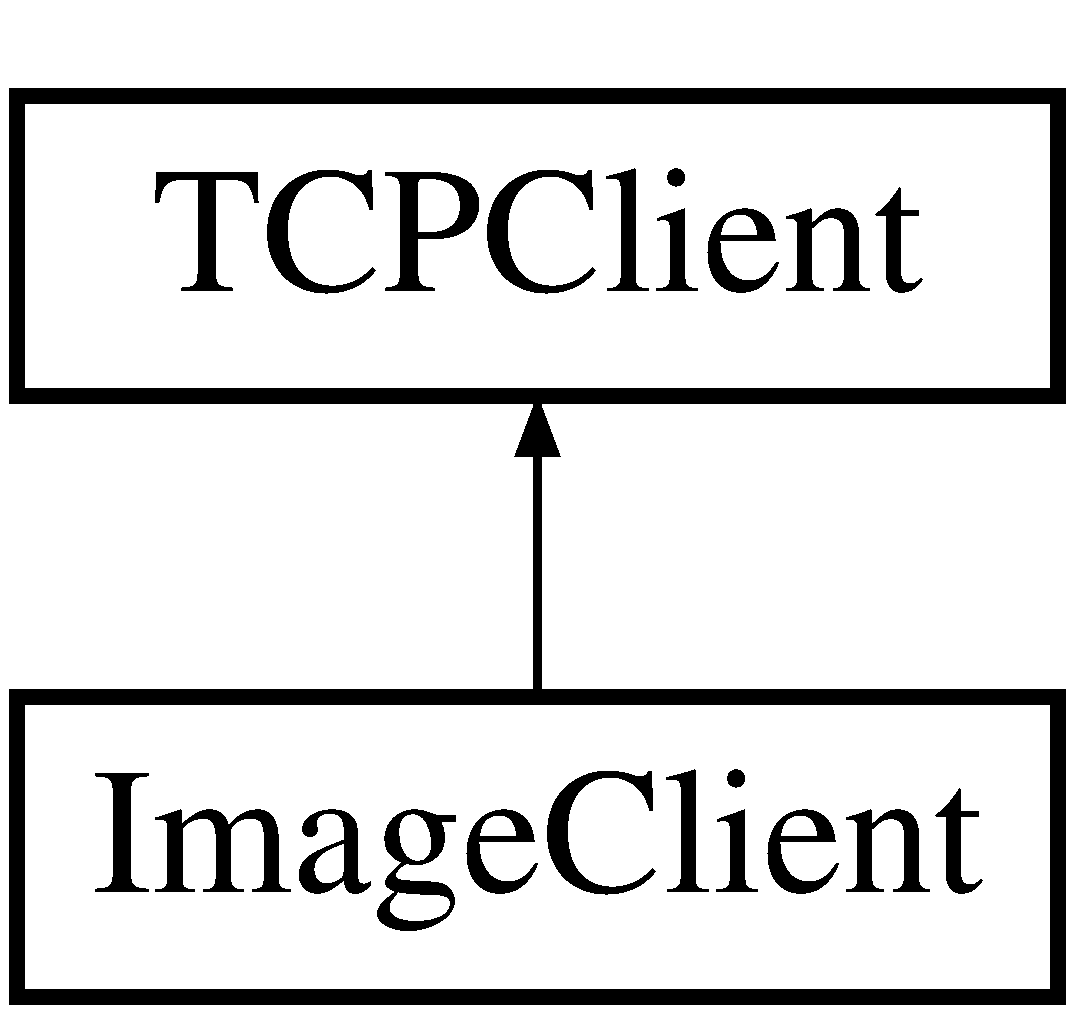
\includegraphics[height=2.000000cm]{classTCPClient}
\end{center}
\end{figure}
\subsection*{Public Member Functions}
\begin{DoxyCompactItemize}
\item 
\hyperlink{classTCPClient_a57b75116cbba7c8b50e26e78642f0d56}{T\-C\-P\-Client} (int serv\-\_\-port, std\-::string serv\-\_\-addr)
\begin{DoxyCompactList}\small\item\em Constructeur permettant d'initialiser les variables utiles pour la connexion au serveur. \end{DoxyCompactList}\item 
\hypertarget{classTCPClient_a869a5b3319ca562d03cb4c59ebec4407}{virtual \hyperlink{classTCPClient_a869a5b3319ca562d03cb4c59ebec4407}{$\sim$\-T\-C\-P\-Client} ()}\label{classTCPClient_a869a5b3319ca562d03cb4c59ebec4407}

\begin{DoxyCompactList}\small\item\em Destructeur standard. \end{DoxyCompactList}\item 
\hypertarget{classTCPClient_a2c3b52fb65b17db330ce851a1111c221}{void \hyperlink{classTCPClient_a2c3b52fb65b17db330ce851a1111c221}{init\-Socket} ()}\label{classTCPClient_a2c3b52fb65b17db330ce851a1111c221}

\begin{DoxyCompactList}\small\item\em Fonction permettant d'initier le socket de communication et établir la connexion avec le serveur. \end{DoxyCompactList}\item 
\hypertarget{classTCPClient_a2acc4f58389c670672c6373b5375cb36}{int \hyperlink{classTCPClient_a2acc4f58389c670672c6373b5375cb36}{get\-Comm\-Socket} () const }\label{classTCPClient_a2acc4f58389c670672c6373b5375cb36}

\begin{DoxyCompactList}\small\item\em Fonction permettant d'obtenir le descripteur du socket de communication. \end{DoxyCompactList}\end{DoxyCompactItemize}


\subsection{Detailed Description}
\textbackslash{} class \hyperlink{classTCPClient}{T\-C\-P\-Client} \hyperlink{classTCPClient}{T\-C\-P\-Client} est une classe de base qui fournit des méthodes permettant d'initier une connexion T\-C\-P/\-I\-P côté client. 

\subsection{Constructor \& Destructor Documentation}
\hypertarget{classTCPClient_a57b75116cbba7c8b50e26e78642f0d56}{\index{T\-C\-P\-Client@{T\-C\-P\-Client}!T\-C\-P\-Client@{T\-C\-P\-Client}}
\index{T\-C\-P\-Client@{T\-C\-P\-Client}!TCPClient@{T\-C\-P\-Client}}
\subsubsection[{T\-C\-P\-Client}]{\setlength{\rightskip}{0pt plus 5cm}T\-C\-P\-Client\-::\-T\-C\-P\-Client (
\begin{DoxyParamCaption}
\item[{int}]{serv\-\_\-port, }
\item[{std\-::string}]{serv\-\_\-addr}
\end{DoxyParamCaption}
)}}\label{classTCPClient_a57b75116cbba7c8b50e26e78642f0d56}


Constructeur permettant d'initialiser les variables utiles pour la connexion au serveur. 


\begin{DoxyParams}{Parameters}
{\em serv\-\_\-port} & Le port du serveur sur lequel se connecter \\
\hline
{\em serv\-\_\-addr} & L'adresse I\-P du serveur sur lequel se connecter \\
\hline
\end{DoxyParams}


The documentation for this class was generated from the following files\-:\begin{DoxyCompactItemize}
\item 
include/T\-C\-P\-Client.\-h\item 
src/T\-C\-P\-Client.\-cpp\end{DoxyCompactItemize}

\hypertarget{classTCPServer}{\section{T\-C\-P\-Server Class Reference}
\label{classTCPServer}\index{T\-C\-P\-Server@{T\-C\-P\-Server}}
}
Inheritance diagram for T\-C\-P\-Server\-:\begin{figure}[H]
\begin{center}
\leavevmode
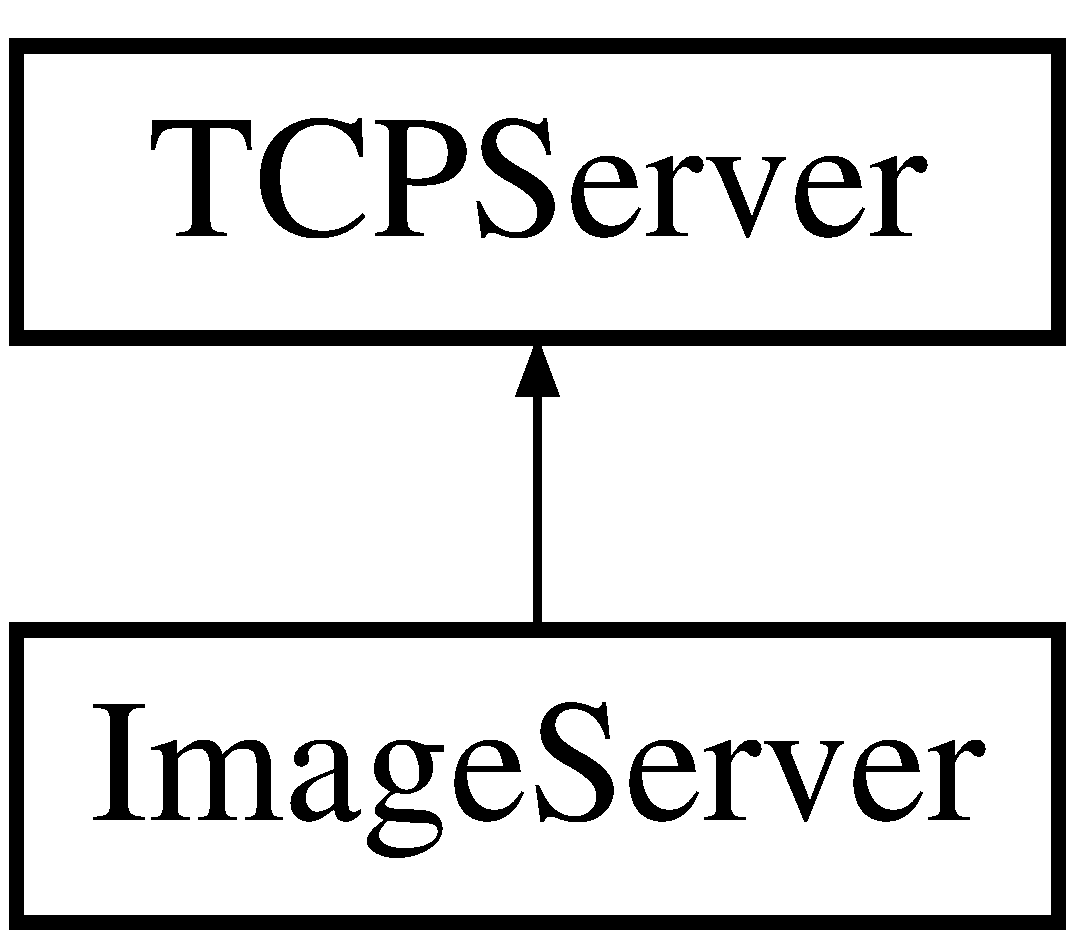
\includegraphics[height=2.000000cm]{classTCPServer}
\end{center}
\end{figure}
\subsection*{Public Member Functions}
\begin{DoxyCompactItemize}
\item 
\hypertarget{classTCPServer_a7d5e52f194a5aba475977cc2b76329c2}{{\bfseries T\-C\-P\-Server} (int port)}\label{classTCPServer_a7d5e52f194a5aba475977cc2b76329c2}

\item 
\hypertarget{classTCPServer_a603f6260d94733c013901736607daf98}{void {\bfseries init\-Socket} ()}\label{classTCPServer_a603f6260d94733c013901736607daf98}

\item 
\hypertarget{classTCPServer_a754871b150fd6dee7fef3b631e81b0fb}{int {\bfseries get\-Comm\-Socket} () const }\label{classTCPServer_a754871b150fd6dee7fef3b631e81b0fb}

\end{DoxyCompactItemize}


The documentation for this class was generated from the following files\-:\begin{DoxyCompactItemize}
\item 
include/T\-C\-P\-Server.\-h\item 
src/T\-C\-P\-Server.\-cpp\end{DoxyCompactItemize}

\hypertarget{structtiming}{\section{timing Struct Reference}
\label{structtiming}\index{timing@{timing}}
}
\subsection*{Public Attributes}
\begin{DoxyCompactItemize}
\item 
\hypertarget{structtiming_a3d4e62541518d2d7090bb7c986fb798f}{int {\bfseries res\-X}}\label{structtiming_a3d4e62541518d2d7090bb7c986fb798f}

\item 
\hypertarget{structtiming_af0dad6c92b1ce60b5f1421fb0928f28a}{int {\bfseries res\-Y}}\label{structtiming_af0dad6c92b1ce60b5f1421fb0928f28a}

\item 
\hypertarget{structtiming_a0db1b574e8a0c4f479fda997891349be}{double {\bfseries fps}}\label{structtiming_a0db1b574e8a0c4f479fda997891349be}

\end{DoxyCompactItemize}


The documentation for this struct was generated from the following file\-:\begin{DoxyCompactItemize}
\item 
src/livrable1.\-cpp\end{DoxyCompactItemize}

%--- End generated contents ---

% Index
\newpage
\phantomsection
\addcontentsline{toc}{part}{Index}
\printindex

\end{document}
